\section{Vorgehensmodelle}

\begin{defi}{Vorgehensmodelle}
    Man sollte die gesamte Vorgehensweise nicht bei jedem Projekt neu erfinden, sondern sich auf vorhandene Erfahrungen abstützen.

    Prinzipien:
    \begin{itemize}
        \item \emph{Planung und Koordination}:

              Alle Beteiligten wissen im Voraus, was getan werden muss.
        \item \emph{Iteration}:

              Das Projekt bringt in kurzen Abständen einsetzbare Versionen (Prototypen) hervor.
        \item \emph{Kontinuierliche Verbesserung}:

              Unvermeidlich auftretende Fehler sollen gut ausgeglichen werden.
    \end{itemize}

    Durch diese Prinzipien soll das Softwareprodukt im gesamten besser werden, da
    \begin{itemize}
        \item eine höhere Qualität,
        \item effizientere Produktion, sowie
        \item bessere Wartbarkeit
    \end{itemize}
    erreicht werden kann.

    Zusätzlich wird der Entwicklungsprozess transparent
    \begin{itemize}
        \item planbarer,
        \item nachvollziehbarer,
        \item kontrollierbarer und
        \item lehrbar.
    \end{itemize}

    Um ein \emph{Vorgehensmodell} zu erstellen, definiert man zuerst verschiedene Phasen.
    Diese werden dann gewichtet, angeordnet und durchlaufen.
    Dabei ist dieses Modell ideal, und meist nicht der Realität exakt entsprechend.
\end{defi}

\begin{defi}{Phase}
    Eine \emph{Phase} ist eine zeitlich begrenzte Aktivität mit einer speziellen Aufgabe, die von Mitarbeitenden mit geeigneten Rollen bearbeitet wird.
    Hierbei sollen basierend auf vorgegebenen Artefakten neue, definierte Artefakte produziert werden.
    Zu einem Zeitpunkt wird immer nur genau eine Phase durchlaufen.
\end{defi}

\begin{defi}{Wasserfallmodell}
    Ein erster Versuch eines sequentiellen Vorgehensmodells ist das \emph{Wasserfallmodell}.

    Dieses klassische Vorgehensmodell funktioniert jedoch in der realen Welt nicht\footnote{Siehe \href{https://res.infoq.com/articles/scaling-software-agility/en/resources/ch02.pdf}{https://res.infoq.com/articles/scaling-software-agility/en/resources/ch02.pdf}}.

    \begin{center}
        \includegraphics[width=0.85\textwidth]{includes/figures/defi_waterfall_model.pdf}
    \end{center}

    \begin{itemize}
        \item Vorteile:
              \begin{itemize}
                  \item Plan auch für NichtexpertInnen verständlich
                  \item einfache Planung
              \end{itemize}
        \item Nachteile:
              \begin{itemize}
                  \item Anforderungen müssen 100\% abgeschlossen sein
                  \item Auftraggebender ist nur in der ersten Phase eingebunden
                  \item Entwicklungsrisiken werden spät erkannt
                  \item Lauffähige Version des Systems erst am Ende
                  \item Zeitverzug im Projekt geht oft zu Lasten späterer Phasen (z.B. beim Testen)
                  \item Testen nur am Ende vorgesehen
              \end{itemize}
    \end{itemize}

    Trotz dieser immensen Nachteilen ist das Wasserfallmodell eines der verbreitesten Modelle.
\end{defi}

\begin{bonus}{Anforderungsanalyse (Wasserfallmodell)}
    Um eine Anforderung zu definieren muss man zuerst das Problem analysieren:
    \begin{itemize}
        \item \emph{Kernprobleme bestimmen}:
              \begin{itemize}
                  \item Welche Funktionen soll das System anbieten?
                  \item Wie soll sich die Benutzungsoberfläche verhalten?
                  \item Wie effizient, sicher etc. muss das System sein?
              \end{itemize}
        \item \emph{relevantes Umfeld bestimmen}:
              \begin{itemize}
                  \item Art, Anzahl der Nutzenden
                  \item Art, Variation der Eingaben
                  \item vorgesehene Hardware, vorhandene Softwareprodukt
              \end{itemize}
        \item \emph{Durchführbarkeit abschätzen}
              \begin{itemize}
                  \item technische, persönliche Kapazität
                  \item Kosten (und Nutzen)
              \end{itemize}
    \end{itemize}
\end{bonus}

\begin{bonus}{Entwurf (Wasserfallmodell)}
    Um die Architektur zu modellieren bzw. das Design festzulegen, muss man:
    \begin{itemize}
        \item das System grob in Komponenten zerlegen
              \begin{itemize}
                  \item Zweck und Rollen einer Komponente
                  \item von einer Komponente angebotene Dienste
              \end{itemize}
        \item ein Zusammenspiel zwischen den Komponenten definieren
              \begin{itemize}
                  \item Welche Abhängigkeiten zwischen Komponenten existieren?
              \end{itemize}
        \item den Entwurf mit den Anforderungen abgleichen
    \end{itemize}
\end{bonus}

\begin{bonus}{Implementierung (Wasserfallmodell)}
    \begin{itemize}
        \item Komponenten implementieren
              \begin{itemize}
                  \item Datenstrukturen wählen
                  \item Algorithmen wählen
                  \item In Programmiersprache formulieren
              \end{itemize}
        \item Komponenten dokumentieren
              \begin{itemize}
                  \item Wie erledigt die Komponente ihre Aufgabe?
                  \item Implementierungsalternativen begründen
              \end{itemize}
        \item Komponenten prüfen und mit den Anforderungen abgleichen
              \begin{itemize}
                  \item Testumgebung einrichten, Testdaten erfassen
                  \item Testläufe durchführen und verifizieren
              \end{itemize}
    \end{itemize}
\end{bonus}

\begin{bonus}{Integration (Wasserfallmodell)}
    \begin{itemize}
        \item Komponenten (zu Paketen) zusammenfügen
        \item Zusammenspiel zwischen den Komponenten prüfen
              \begin{itemize}
                  \item Funktionalität prüfen
                  \item Effizienz, Sicherheit nach Anforderung überprüfen
              \end{itemize}
    \end{itemize}
\end{bonus}

\begin{bonus}{Installation bzw. Auslieferung (Wasserfallmodell)}
    \begin{itemize}
        \item System beim Auftraggebenden installieren
        \item Daten migrieren
        \item Anpassen
        \item Altsystem deinstallieren
        \item Abnahmen durch Auftraggebenden
        \item Benutzenden schulen
    \end{itemize}
\end{bonus}

\begin{bonus}{Wartung (Wasserfallmodell)}
    Die am meisten unterschätze Phase in Vorgehensmodellen ist die Wartung.
    Dabei stellt diese mit knapp 70\% des Arbeitsaufwands den Großteil des z.B. Wasserfallmodells dar.

    \begin{itemize}
        \item Fehler beheben
              \begin{itemize}
                  \item algorithmische Fehler
                  \item Fehler bezüglich der Anforderungen
              \end{itemize}
        \item Modifizieren
              \begin{itemize}
                  \item Auf andere Hardware portieren
                  \item Funktionalität erweitern / verbessern
              \end{itemize}
    \end{itemize}
\end{bonus}

\begin{defi}{Prototypische Entwicklung}
    Ein neuer Ansatz für Vorgehensmodelle bzw. eine Weiterentwicklung des Wasserfallmodells ist die \emph{Prototypische Entwicklung}.

    \begin{center}
        \includegraphics[width=0.85\textwidth]{includes/figures/defi_prototype_development.pdf}
    \end{center}

    \begin{itemize}
        \item Vorteile:
              \begin{itemize}
                  \item frühzeitige Risikominimierung durch frühzeitige Erkennung potenzieller Probleme
                  \item Schnelles erstes Projektergebnis
              \end{itemize}
        \item Nachteile:
              \begin{itemize}
                  \item Anforderungen müssen 100\%-tig sein
                  \item KundIn erwartet schnell Endergebnis
              \end{itemize}
    \end{itemize}
\end{defi}

\begin{defi}{Iterative Entwicklung}
    \begin{wrapfigure}{r}{0.4\textwidth}
        \centering
        \includegraphics[width=0.5\textwidth]{includes/figures/defi_iterative_development.pdf}
    \end{wrapfigure}

    Eine Weiterentwicklung der Prototypidee ist die \emph{iterative Entwicklung}.
    Hierbei wird das System in jeder Iteration bis zum fertigen Produkt verfeinert.

    In der ersten Iteration wird daher der Schwerpunkt auf Analyse und Machbarkeit gelegt.
    Später wird auf die Realisierung geachtet.

    \begin{itemize}
        \item (große) Vorteile:
              \begin{itemize}
                  \item dynamische Reaktion auf Risiken
                  \item Teilergebnisse mit KundInnen diskutierbar
              \end{itemize}
        \item Nachteile:
              \begin{itemize}
                  \item schwierige Projektplanung
                  \item schwierige Vertragssituation
                  \item KundIn erwartet zu schnell Endergebnisse
                  \item KundIn sieht Anforderungen als beliebig änderbar
              \end{itemize}
    \end{itemize}
\end{defi}

\begin{example}{Iterative Entwicklung}
    \begin{center}
        \includegraphics{includes/figures/example_iterative_development.pdf}
    \end{center}
\end{example}

\begin{defi}{Inkrementelle Entwicklung}
    Im Gegensatz zur iterativen Entwicklung konzentriert man sich bei der \emph{inkrementellen Entwicklung} primär auf die Kernanforderungen.

    Nach der Anforderungsanalyse erstellt man ein vollständiges Produktmodell und implementiert dementsprechend einen ersten Prototypen mit den relevantesten Funktionen.
    Diese Kern bzw. Null-Version beinhaltet circa 10\% der vollständigen Funktionalitäten, ist jedoch für die Kernaufgaben voll funktional.

    Mit diesem Prototyp sammeln Anwendende Erfahrungen und Wünsche, welche dem Kernsystem hinzugefügt werden.

    \begin{itemize}
        \item Vorteile
              \begin{itemize}
                  \item KundInnen erhalten vorab Zugang zu den (voll implementierten) Funktionen, welche am stärksten benötigt werden
              \end{itemize}
        \item Nachteile
              \begin{itemize}
                  \item Anforderungen müssen erneut 100\%ig sein
                  \item KundInnen konzentrieren sich eher auf fehlende Features anstatt auf das gesamte Produkt
              \end{itemize}
    \end{itemize}
\end{defi}

\begin{example}{Inkrementelle Entwicklung}
    \begin{center}
        \includegraphics{includes/figures/example_incremental_development.pdf}
    \end{center}
\end{example}

\begin{defi}{Iterativ Inkrementelle Entwicklung}
    Bei diesem meist intuitiv genutzten Vorgehensmodell wird das Projekt in kleine Teilschritte zerlegt.
    Hierbei erhält man nach jedem Schritt eine neue Funktionalität (Inkrement).
    Zusätzlich werden existierende Ergebnisse überarbeitet (Iteration).
    Dabei kann man die Probleme des aktuellen Schritts im Folgeschritt lösen.
\end{defi}

\begin{bonus}{Boehmsches Spiralmodell}
    Die Hauptidee des \emph{Boehmschen Spiralmodells} ist es das größte Risiko zu beseitigen.
    So wird jeder Zyklus des Wasserfall-Modells iterativ mehrfach durchlaufen.
    Dadurch nähert sich das Projekt über einen längeren Zeitraum den jeweiligen Zielen an.
    Hierbei finden vermehrt Risikoanalysen wie Verifikationen und Validationen statt.

    Da die Phasen iterativ durchlaufen werden, kann man das Boehmsche Spiralmodell als iterative Vorgehensweise beschreiben.
    Jedoch ist nach einem Zyklus die Phase abgeschlossen, also ein Inkrement, beispielsweise ein Prototyp, fertig.
    Dadurch vermischt es diese beiden Vorangehensweisen miteinander.

    \begin{center}
        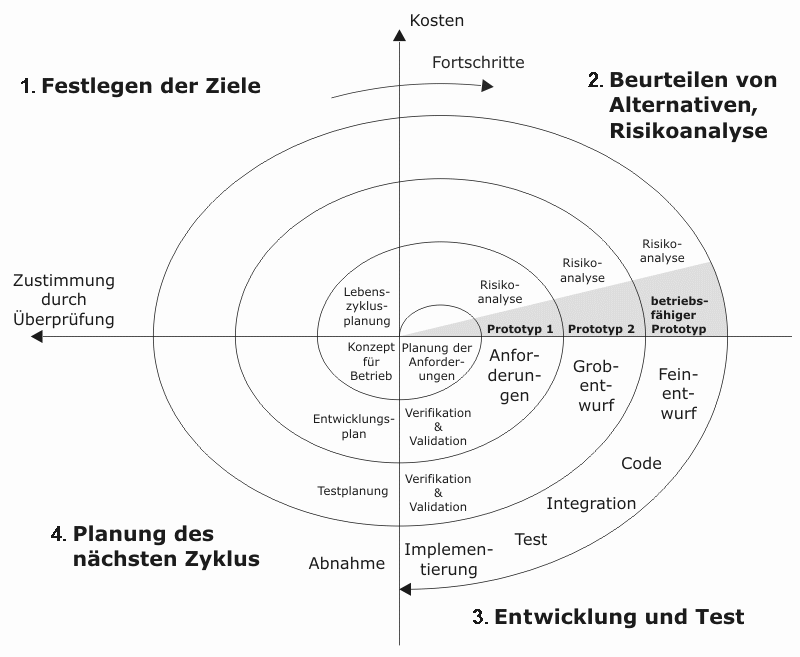
\includegraphics[width=0.75\textwidth]{includes/figures/bonus_boehmsches_spiralmodell.png}
    \end{center}
\end{bonus}

\begin{defi}{V-Modell}
    \includegraphics[width=\textwidth]{includes/figures/defi_v_model.pdf}

    Das \emph{V-Modell} kann iterativ oder inkrementell zu einem W-Modell\footnote{Zwei aneinandergereihte V-Modelle} erweitert werden.

    Historie:
    \begin{itemize}
        \item Das \emph{V-Modell 92} ergänzt das Wasserfallmodell mit Aktivitäten und Ergebnissen
        \item Das \emph{V-Modell 97} fügt inkrementelle Ideen zu noch früheren Anforderungen zu
        \item Das \emph{V-Modell XT} (eXtreme Tailoring) legt weiterhin größeren Fokus auf das Verhältnis zwischen Auftraggebenden und Auftragnehmenden.
    \end{itemize}
\end{defi}

\begin{defi}{RUP}
    Ein weiteres Vorgehensmodell wird durch den \emph{Rational Unified Process} beschrieben.

    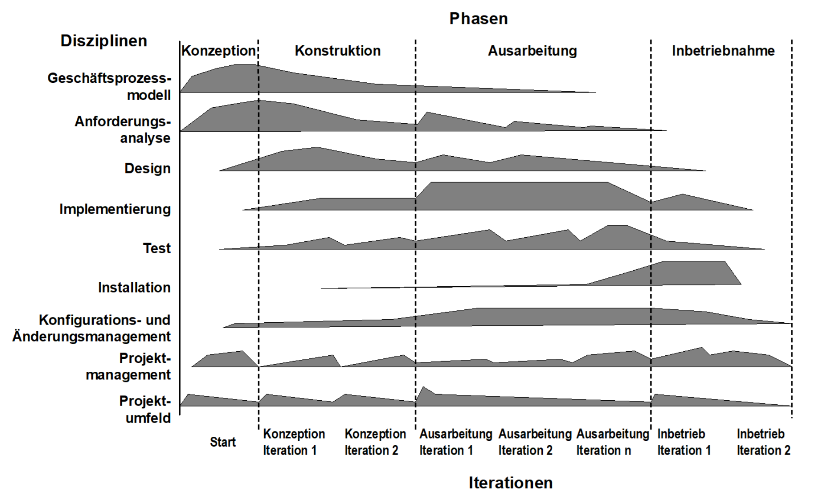
\includegraphics[width=\textwidth]{includes/figures/defi_RUP.png}
\end{defi}

\begin{bonus}{Konzeption (RUP)}
    \begin{itemize}
        \item Ermittlung zentraler Anforderungen
        \item Projektumfang definieren
        \item erste Entwurfs und Implementierungsansätze
        \item Identifikation der Projektrisiken und Aufwände
    \end{itemize}
\end{bonus}

\begin{bonus}{Konstruktion (RUP)}
    \begin{itemize}
        \item Implementierung
        \item Integration
        \item auslieferbare Version
    \end{itemize}
\end{bonus}

\begin{bonus}{Ausarbeitung (RUP)}
    \begin{itemize}
        \item stabile, möglichst vollständige Anforderungen
        \item Entwurfsspezifikation
        \item detaillierter Projektplan mit aktiven Risikomanagement
    \end{itemize}
\end{bonus}

\begin{bonus}{Inbetriebnahme (RUP)}
    \begin{itemize}
        \item Beta-Test
        \item Endabnahme
        \item Inbetriebnahme
        \item Endlieferung
    \end{itemize}
\end{bonus}

% \begin{bonus}{RUP Struktur}
%     \includegraphics[width=\textwidth]{includes/figures/RUP_structure.png}
% \end{bonus}

\begin{bonus}{Kritik an Vorgehensmodellen}
    \begin{itemize}
        \item Es müssen viele Dokumente erzeugt und gepflegt werden.
        \item Eigene Wissenschaft, Modelle wie V-Modelle und RUP zu verstehen und zurecht zu schneiden
        \item Prozessbeschreibung hemmen Kreativität
        \item Anpassung an neue Randbedingungen, z.B. neue Technologien (Web-Services) in Prozessen und benutzten Werkzeugen ist extrem aufwändig.
    \end{itemize}
\end{bonus}

\begin{defi}{SCRUM}
    \emph{SCRUM} ist ein Vorgehensmodell des Projekt- und Produktmanagements, insbesondere zur agilen Softwareentwicklung.

    Grundideen von SCRUM\footnote{eng. für \enquote{Gedränge}}:
    \begin{itemize}
        \item Rollen
              \begin{itemize}
                  \item Product Owner
                        \begin{itemize}
                            \item Definiert Produkt Features\footnote{Inhalt des Product Backlogs} inkl. Priorisierung bei potentiell jedem Sprint
                            \item Bestimmt Auslieferungsdatum, Inhalt sowie finanzielle Ergebnisse
                            \item Akzeptiert oder weist Arbeitsergebnisse zurück
                        \end{itemize}
                  \item Scrum Master
                        \begin{itemize}
                            \item Verantwortlich für Einhaltung von Scrum-Werten und -Techniken
                            \item Stellt sicher, dass Team vollständig funktional und produktiv ist
                            \item Unterstützt enge Zusammenarbeit zwischen allen Rollen und Funktionen
                        \end{itemize}
                  \item Das Team
                        \begin{itemize}
                            \item Typischerweise 5-9 Vollzeitmitglieder
                            \item Funktionsübergreifend (QS, Programmierung, UI-Design etc.)
                            \item Teams organisieren sich selbst
                            \item Mitgliedschaft kann sich nur zwischen Sprints verändern
                        \end{itemize}
              \end{itemize}
        \item Meetings
              \begin{itemize}
                  \item Sprint-Planung
                  \item Sprint-Review
                  \item Sprint-Retrospektive
                  \item Tägliches 15-minütiges Scrum-Meeting
                        \begin{itemize}
                            \item Was hast du gestern getan?
                            \item Was wirst du heute tun?
                            \item Welche Hindernisse sind in deinem Weg?
                        \end{itemize}
              \end{itemize}
        \item Artefakte
              \begin{itemize}
                  \item Product Backlog
                        \begin{itemize}
                            \item Eine Liste \emph{aller} gewünschten Projektarbeiten basierend auf den Anforderungen
                        \end{itemize}
                  \item Sprint Backlog
                        \begin{itemize}
                            \item Eine Liste \emph{der aktuell zu bearbeitenden} Projektarbeiten des Sprints
                        \end{itemize}
                  \item Burndown-Diagramm bzw. Stundensystem
              \end{itemize}
    \end{itemize}
\end{defi}

\begin{bonus}{Aufbau SCRUM}
    Zu Begin jedes Sprints entscheidet sich der \emph{Product Owner} für ein Feature vom \emph{Product Backlog}.
    Für dieses Feature wird ein Sprint (2-4 Wochen) angelegt, welches ein auslieferbares Inkrement der Software erstellt.
    In diesem Zeitraum finden täglich \emph{15-minütige Meetings} statt.

    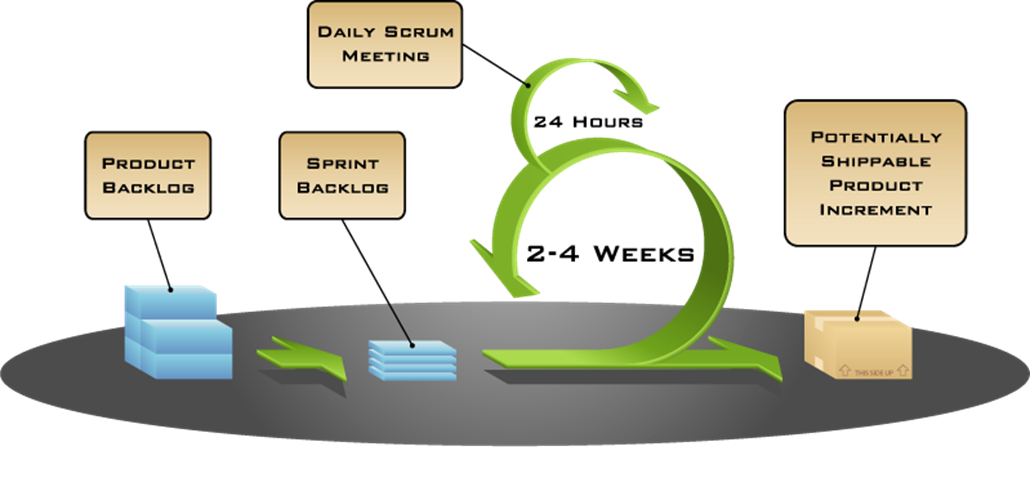
\includegraphics[width=\textwidth]{includes/figures/bonus_SCRUM.png}
\end{bonus}